\section{Funciones de costo componentes ADCS}
\label{ap:Z9}


\begin{figure*}[h]
	\centering
	\begin{subfigure}[t]{0.6\textwidth}
		\centering{%
			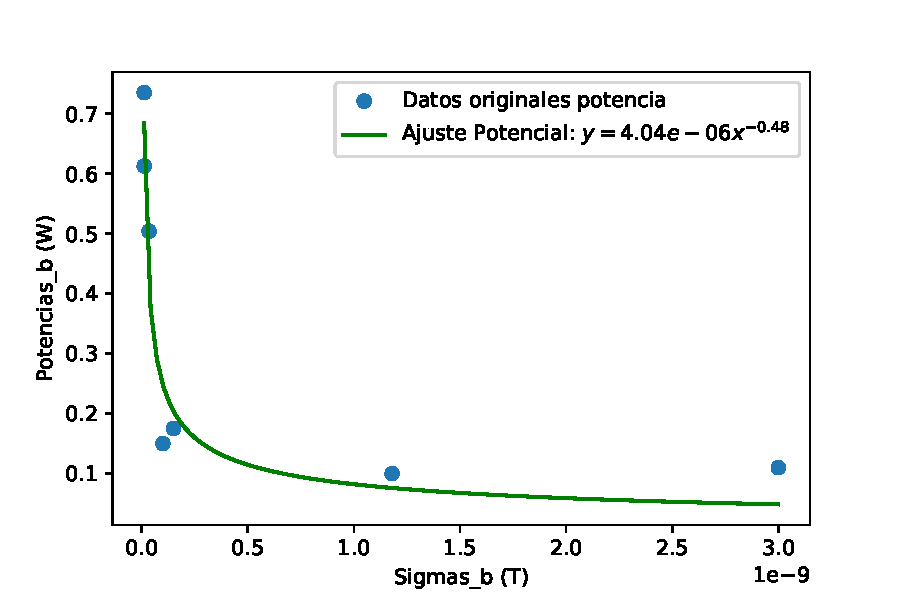
\includegraphics[width=\textwidth]{potencia_magn.pdf}
		}%
		\subcaption{Gráfica desviación estándar vs potencia promedio de los magnetómetros.\label{fig:pot_magn}}
	\end{subfigure}
	\begin{subfigure}[t]{0.6\textwidth}
		\centering{%
			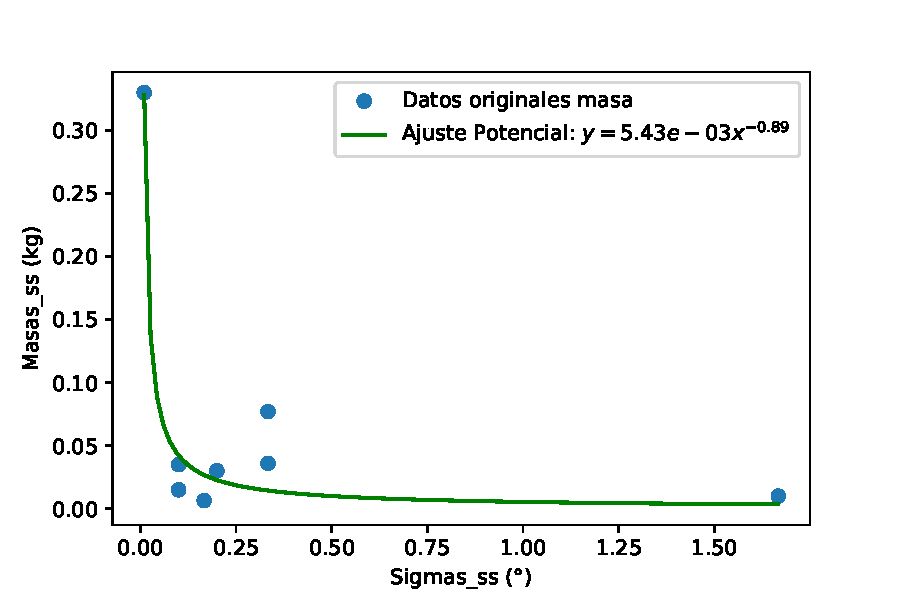
\includegraphics[width=\textwidth]{masa_ss.pdf}
		}%
		\subcaption{Gráfica desviación estándar vs masa de los magnetómetros.\label{fig:masa_magn}}
	\end{subfigure}
	\caption{Datos de masa y potencia promedio de magnetometros y su ajuste potencial.}\label{fig:magn_aj}
\end{figure*}

\begin{figure*}[h]
	\centering
	\begin{subfigure}[t]{0.6\textwidth}
		\centering{%
			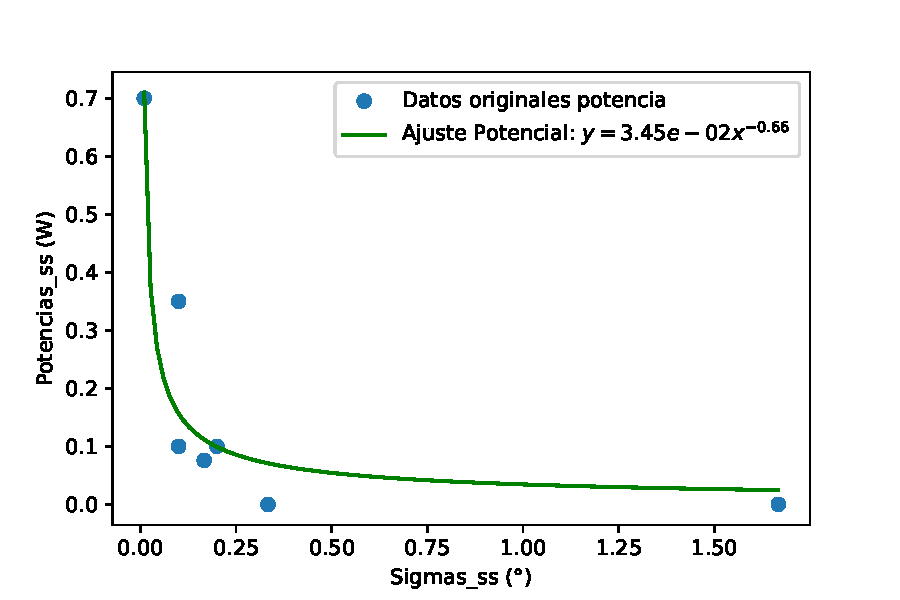
\includegraphics[width=\textwidth]{potencia_ss.pdf}
		}%
		\subcaption{Gráfica desviación estándar vs potencia promedio de los sensores de sol.\label{fig:pot_ss}}
	\end{subfigure}
	\begin{subfigure}[t]{0.6\textwidth}
		\centering{%
			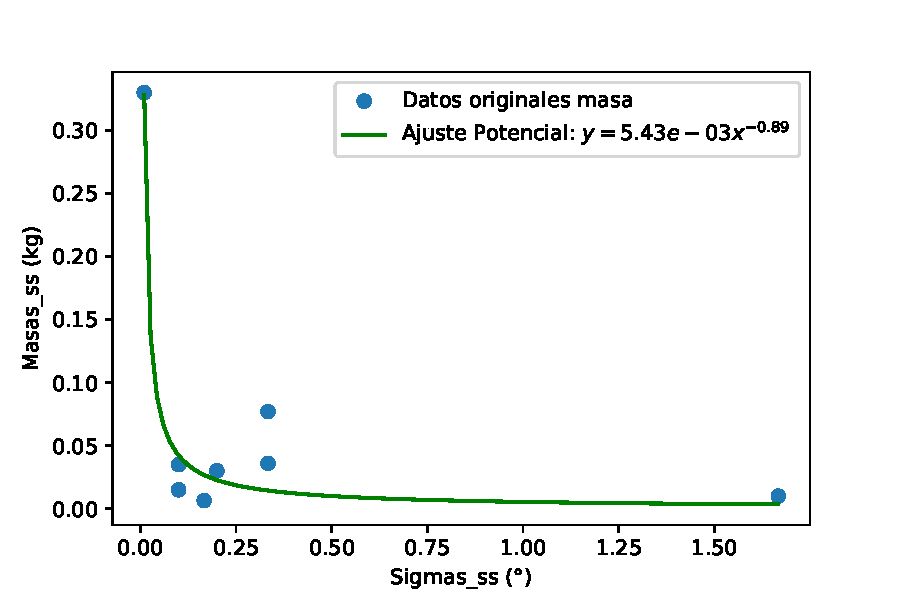
\includegraphics[width=\textwidth]{masa_ss.pdf}
		}%
		\subcaption{Gráfica desviación estándar vs masa de los sensores de sol.\label{fig:masa_ss}}
	\end{subfigure}
	\caption{Datos de masa y potencia promedio de sensores de sol y su ajuste potencial.}\label{fig:ss_aj}
\end{figure*}


\begin{figure*}[h]
	\centering
	\begin{subfigure}[t]{0.6\textwidth}
		\centering{%
			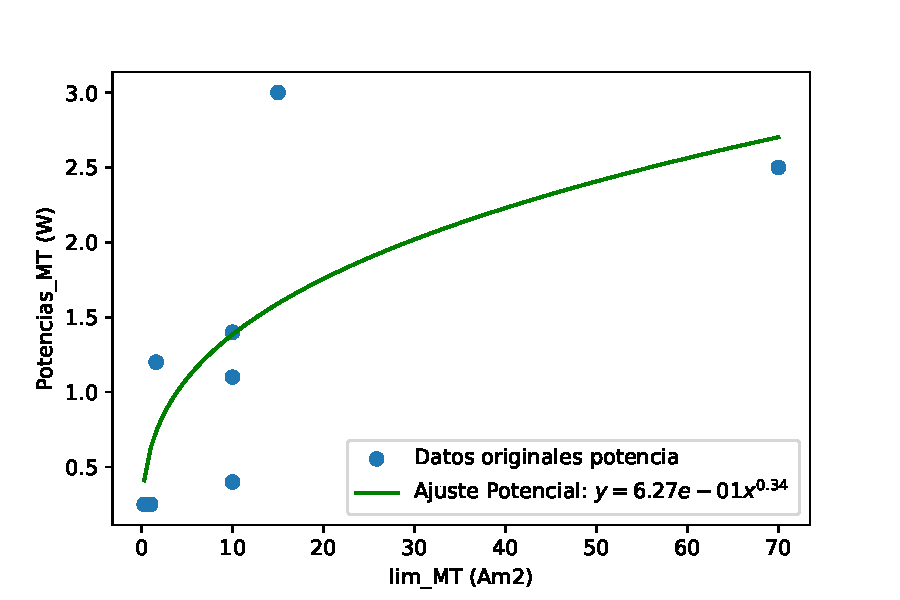
\includegraphics[width=\textwidth]{potencia_MT.pdf}
		}%
		\subcaption{Gráfica límite de actuador vs potencia promedio de los magnetorquers.\label{fig:pot_MT}}
	\end{subfigure}
	\begin{subfigure}[t]{0.6\textwidth}
		\centering{%
			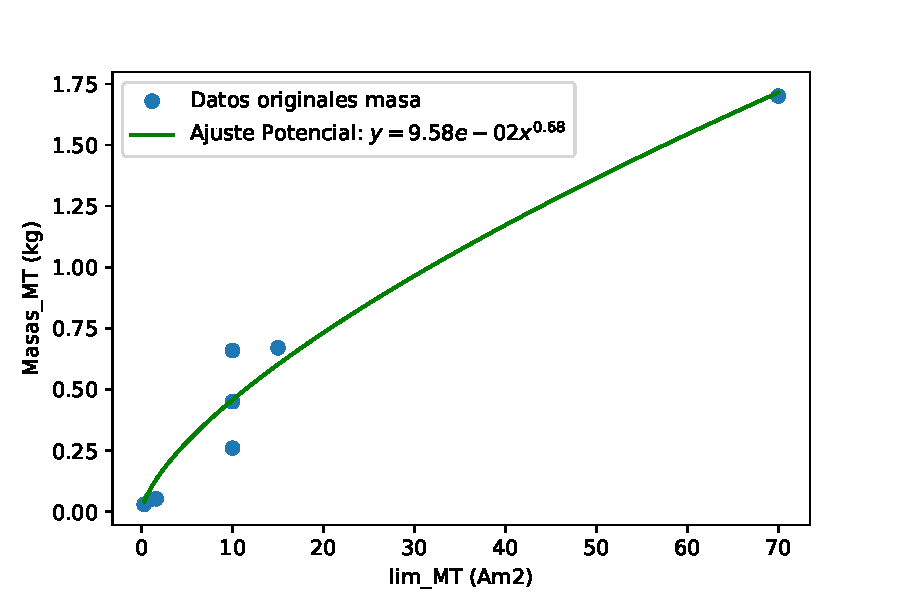
\includegraphics[width=\textwidth]{masa_MT.pdf}
		}%
		\subcaption{Gráfica límite de actuador vs masa de los magnetorquers.\label{fig:masa_MT}}
	\end{subfigure}
	\caption{Datos de masa y potencia promedio de magnetorquers y su ajuste potencial.}\label{fig:MT_aj}
\end{figure*}


\begin{figure*}[h]
	\centering
	\begin{subfigure}[t]{0.6\textwidth}
		\centering{%
			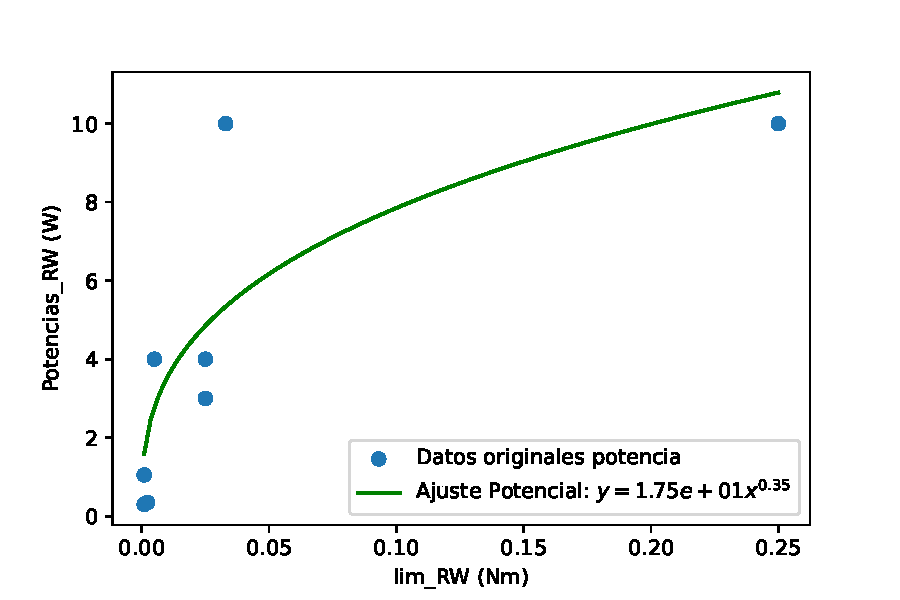
\includegraphics[width=\textwidth]{potencia_RW.pdf}
		}%
		\subcaption{Gráfica limite de actuador vs potencia promedio de las ruedas de reacción.\label{fig:pot_RW}}
	\end{subfigure}
	\begin{subfigure}[t]{0.6\textwidth}
		\centering{%
			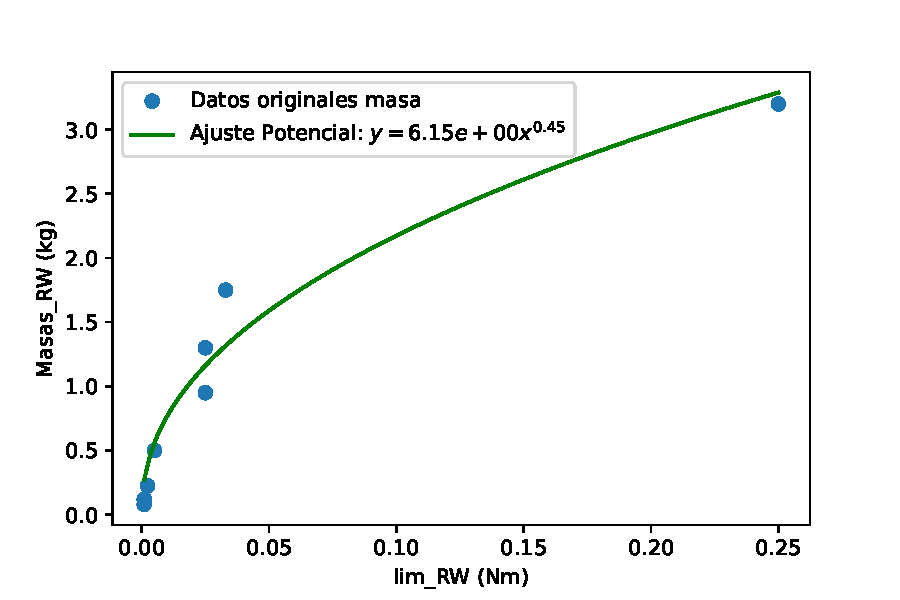
\includegraphics[width=\textwidth]{masa_RW.pdf}
		}%
		\subcaption{Gráfica límite de actuador vs masa de las ruedas de reacción.\label{fig:masa_RW}}
	\end{subfigure}
	\caption{Datos de masa y potencia promedio de ruedas de reacción y su ajuste potencial.}\label{fig: RW_aj}
\end{figure*}
